%&tex
\documentclass{standalone}

\usepackage{graphicx}

\usepackage{cleveref}
\usepackage{subcaption}

\usepackage{tikz}
\usetikzlibrary{arrows,shapes,backgrounds,calc}
\usepackage{bm}

\begin{document}


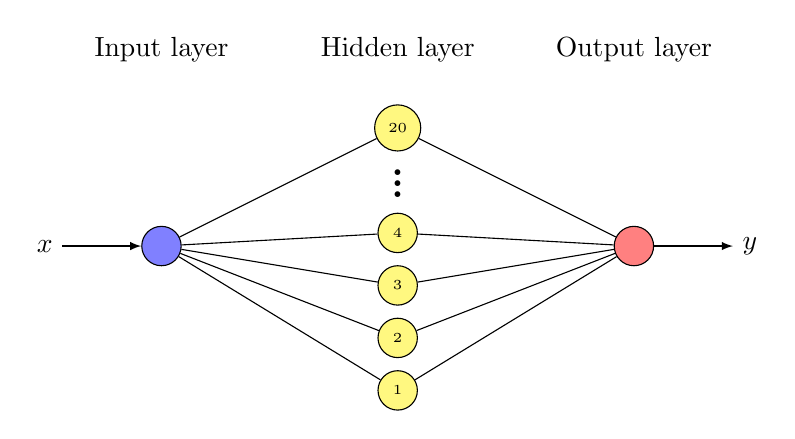
\begin{tikzpicture}

    % % hidden layer neurons
    % \foreach \i in {1,...,2}
    % {
    %     \node[draw,
    %     circle,
    %     minimum size = 0.5 cm,
    %     fill=blue!90] (HL_CD_1-\i)  at (1.5, \i-2.5){};
    %
    %     \node[draw,
    %     circle,
    %     minimum size = 0.5 cm,
    %     fill=green!90] (HL_V_1-\i)  at (1.5, \i-0.5){};
    % }

    % input layer
    \node[draw,
    circle,
    minimum size = 0.5cm,
    fill = blue!50] (X) at (0,0) {};

    % hidden layer
    \foreach \i in {1,...,4}
    {
        \node[draw,
        circle,
        minimum size = 0.5cm,
        fill = yellow!50] (HL-\i) at (3,\i/1.5-2.5){\tiny\i};
    }
    \node[draw,
    circle,
    minimum size = 0.5cm,
    fill = yellow!50] (HL-5) at (3,1.5){\tiny 20};
    \node[] (Dots) at (3,0.9){\Large\(\bm{\vdots}\)};

    % output layer
    \node[draw,
    circle,
    minimum size = 0.5cm,
    fill = red!50] (Y) at (6,0) {};

    % drawing connections
    \foreach \i in {1,...,5}
    {
        \draw (X) -- (HL-\i);
        \draw (Y) -- (HL-\i);
    }
    \draw[latex-] (X.west) -- ++(-1,0) node[left] {$x$};
    \draw[-latex] (Y.east) -- ++(1,0) node[right] {$y$};

    % defining labels
    \node at (0,2.5) {Input layer};
    \node at (3,2.5) {Hidden layer};
    \node at (6,2.5) {Output layer};

\end{tikzpicture}

\end{document}
